\begin{frame}
	\frametitle{Pong original}
	
    \begin{center}
        \textbf{La leyenda}
    \end{center}
	
    \begin{center}
		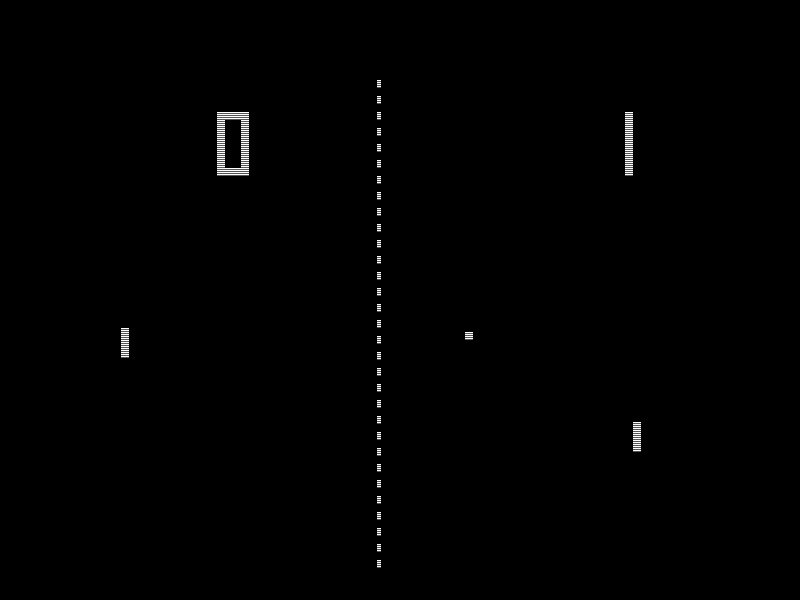
\includegraphics[scale=0.4]{img/pong-original.png}
	\end{center}	

\end{frame}

\begin{frame}
	\frametitle{Pong original}
	
	Para ir abriendo boca:
	
	\begin{columns}[c]
	\column{175pt}
		
	\begin{block}{Pong Facts}
		\begin{itemize}
            \item Uno de los primeros videojuegos de la historia.
			\item Creado por Nolan Bushnell en 1972 para Atari.
            \item Atari demandó a muchísimas copias de Pong.
            \item Tuvo un grandioso éxito... y ahora estamos aquí.
		\end{itemize}            
	\end{block}
	
	\column{125pt}
	
	\begin{center}
		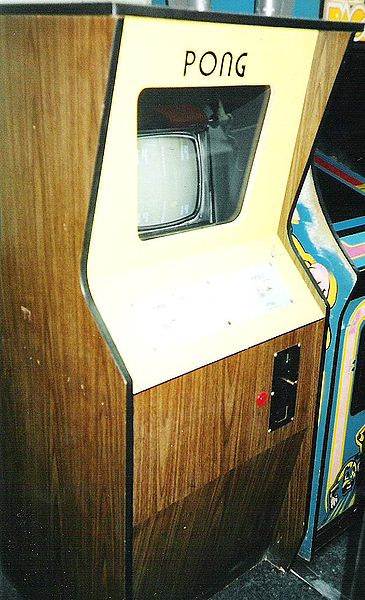
\includegraphics[scale=0.3]{img/pong-recreativa.jpg}
	\end{center}	
	
	\end{columns}
	
\end{frame}

\begin{frame}
	\frametitle{Pong - Diseño}
	
	\begin{center}
	Toca diseñar nuestro Pong, ¡manos a la obra!
	\end{center}
	
	\begin{columns}[c]
	\column{175pt}
		
	Recordad	
	
	\begin{block}{Previously...}
		\begin{itemize}
			\item Planteamiento, concepto y género
			\item Personajes, enemigos y objetos
			\item Mecánicas
		\end{itemize}            
	\end{block}
	
	\column{125pt}
	
	\begin{center}
		
\includegraphics[scale=0.3]{img/Lamp-256.png}
	\end{center}	
	
	\end{columns}
	
	\begin{center}
	Con más más formalidad en el Game Design Document
	\end{center}
	
\end{frame}

\begin{frame}
	\frametitle{Pong - Diseño - Planteamiento}
	
	\begin{columns}[c]
	\column{175pt}	
	
	\begin{block}{Planteamiento}
		\begin{itemize}
			\item Juego arcade
			\item Simulación muy básica del tenis
			\item Jugador VS Inteligencia Artificial
		\end{itemize}            
	\end{block}
	
	\column{125pt}
	
	\begin{center}
		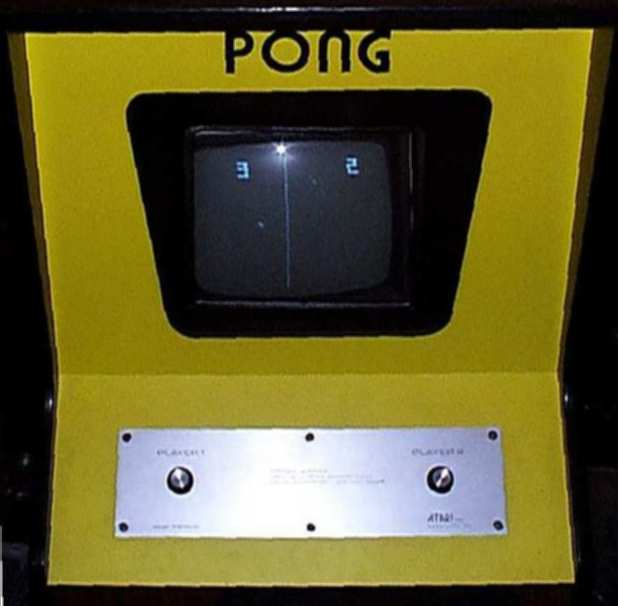
\includegraphics[scale=0.2]{img/pong-recreativa-2.jpg}
	\end{center}
	
	\begin{center}
	    Esta recreativa derrocha amor
	\end{center}	
	
	
	\end{columns}
	
\end{frame}

\begin{frame}
	\frametitle{Pong - Diseño - Mecánica}
	
	\begin{columns}[c]
	\column{175pt}	
	
	\begin{block}{Palas}
		\begin{itemize}
			\item Tablero rectangular
			\item El jugador controla una pala
			\item La IA controla otra pala
			\item Deben golpear una pelota para marcar en el campo contrario
			\item La IA será invencible (survival)
			\item Cada vez que se devuelve la pelota el jugador consigue un punto
			\item Superación del récord
		\end{itemize}            
	\end{block}
	
	\column{125pt}
	
	\begin{center}
		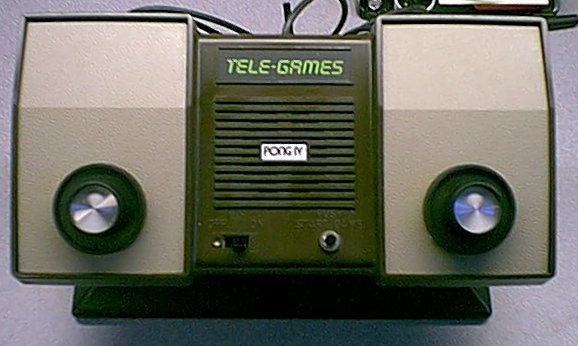
\includegraphics[scale=0.45]{img/telepong.jpg}
	\end{center}
	
	\begin{center}
	    Dos jugadores en el mismo pad
	\end{center}	
	
	\end{columns}
	
\end{frame}

\begin{frame}
	\frametitle{Pong - Diseño - Jugador}
	
	\begin{columns}[c]
	\column{175pt}	
	
	\begin{block}{Jugador humano}
		\begin{itemize}
			\item Movimiento: arriba y abajo
			\item Sin salirse del tablero
		\end{itemize}            
	\end{block}
	
	\column{125pt}
	
	\begin{center}
		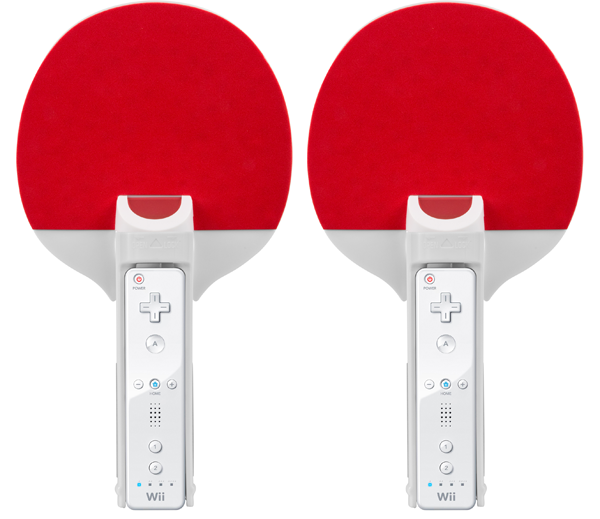
\includegraphics[scale=0.6]{img/wiipong.png}
	\end{center}	
	
	\begin{center}
	Estas \textbf{NO} serán nuestras palas
	\end{center}
	
	\end{columns}
	
\end{frame}

\begin{frame}
	\frametitle{Pong - Diseño - Bola}
	
	\begin{columns}[c]
	\column{175pt}	
	
	\begin{block}{Bola}
		\begin{itemize}
			\item Movimiento rectilíneo uniforme
			\item Rebotes en palas y bordes
			\item No tendremos en cuenta ángulos de choque
		\end{itemize}            
	\end{block}
	
	\column{125pt}
	
	\begin{center}
		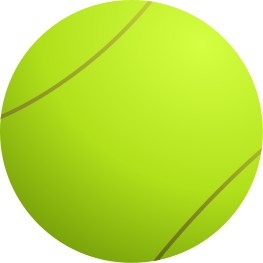
\includegraphics[scale=0.4]{img/pelota.png}
	\end{center}	
	
	\begin{center}
	    Aún no tendremos que desempolvar los libros de física de la ESO
	\end{center}
	
	\end{columns}
	
\end{frame}

